\documentclass{article}
\usepackage[utf8]{inputenc}
\usepackage[top=1in, bottom=1.25in, left=1.25in, right=1.25in]{geometry}
\usepackage{graphicx}




\title{Manging big data with My SQL}
\author{Elias  Altrabsheh}
\date{November 2016}

\begin{document}

\maketitle

\section*{Introduction of course}

This course is a 5 weeks course introducing manging databases using SQL. This will include how to execute the most useful query and table aggregation statements for business analysts, and practice using those queries with real databases. Databases are collections of tables that each have their own unified theme. These tables are linked by one or more columns with the same values. These columns allow you to connect rows in different tables. 

\subsection*{Week 1}
\subsubsection*{Problems Databases Solve}

We start by asking the questions on  Why do we need databases in all this complicated database query language? Why can't businesses keep things simple and just store things in spreadsheets? To examine these statements, We give an example of a business that uses a data sheet.\\

\noindent From the example giving in lecture one we can summarise the following :\\

\textbf{Good data Storage allows}

\begin{itemize}
    \item Easy retrieval 
    \item Easy updating
    \item Accessibility for multiple people at the same time
    \item Data concisest
    \item space efficiency 
    \item speed and security
\end{itemize}

\textbf{How would you design a data storage system that wasn't a single spread sheet?}

\begin{itemize}

    \item date retrieval needs to be as quick as possible and takes up minimal space so we can use relational databases like My SQL. 
    
    \item  if you require to retrrive data it will only call subset of data. rational data base breaks down data into subsets that are kept in its own tables.  A critical piece of database design is making sure each individual table with its own unified theme contains a column with unique values that allows you to link that table to other tables. 
    
    \item set theory and rational algebra is applied to manipulate the data set.  
    
\end{itemize}
\pagebreak

\subsection*{Database Design Tools}
\subsubsection*{How Entity-Relationship Diagrams Work}


\begin{figure}[h]

\centering
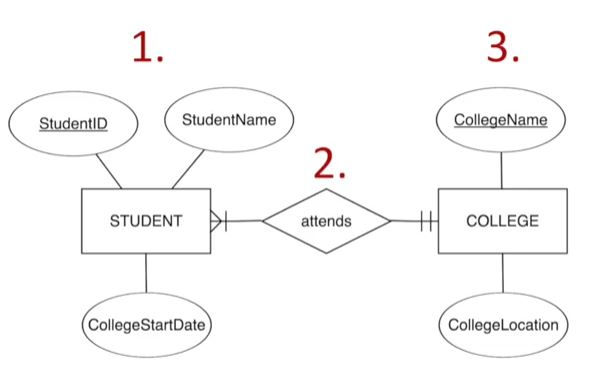
\includegraphics[width=0.7\textwidth]{week1-1}

\caption{entity relationship diagram }
\end{figure}

The boxes in the Diagram are called Entities. They represent categories of data your database will keep track of. Each box is one category. Eventually, each entity will probably become a table when the database is made. \\

The ovals in the Diagram are called Attributes. These represent aspects of each category or entity that will be recorded. Attributes will likely become the columns in the table that will be built around that entity. Each attribute in the Diagram has to be connected to at least one entity. Further, according to the rules of set theory, each attribute must be unique for that entity. So you shouldn't, in theory at least, have two college start dates in your student entity, for example. \\

Each relationship between entities in the Diagram shows how many instances of one entity are associated with how many instances of another entity. \\

There is also the symbol that represents the cardinality that one line represents 1 and two lines represents many. Other than one or many these relationships can have numbers associated with them as:
\textbf{specific cardinality constraint notation}
\begin{itemize}
\item  numbers take precedence over symbols.
\item numbers are always written from left to right.
\end{itemize}
\pagebreak

\subsubsection*{Database Structures Illustrated by Entity-Relationship Diagrams}

\begin{figure}[h]

\centering
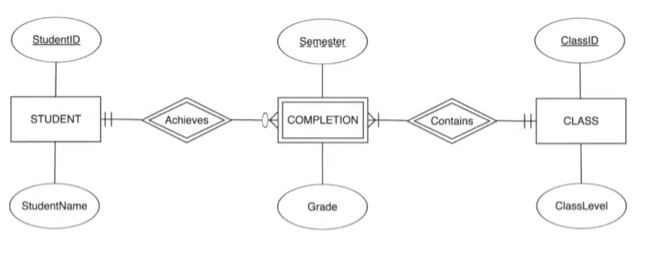
\includegraphics[width=0.9\textwidth]{week1-2}

\caption{entity relationship diagram (more complicated) }
\end{figure}

In general, students are taking group of classes.but student names cant be directly connected to ID in this data base, even though student and class have a unique attribute. They can be connected if you can combine via semester of the class taken in. but that means , students can take class multiple times. This makes the data more complicated as in the query you have to specify multiple tables if the student failed. 

\subsubsection*{Relational Schemes}
\textbf{The critical components of a relation scheme is :}
\begin{itemize}

\item Tables 
\item Primary keys: column or set of columns who value is unique for every row in a table. also only one column per table can be primary key unless multiple column are needed to identify each row.
\item Foreign keys: column or set of columns who value is unique for every row in a table, but can contain null values. It also can be refers to primary keys of another table. A good comment to remember that foreign keys and unique keys cannot have the same name.  
\end{itemize}

A good way to describe relation schemes as a blue prints of database. Which means its a plan for your data base. There is a set of technical terminally to describes these schemes and table , columns and rows are not normally used .
\pagebreak

\section*{Week 2}
\subsection*{Introduction to Query Syntax}
\subsubsection*{Introduction to Query Syntax}
SQL has commands from many different aspects of creating and manipulating a database. But since you're rarely be given information to change stored data as a data analyst, we will exclusively cover DQL or Data Query Language, part of SQL. This part of a language that allows you to retrieve data from the database in whatever format you want.\\

\noindent  \textbf{Querys} are collection of line in SQL that describes the data you want and the format type wanted in. These can be accessed by the front end interface that varies from company to company.  \\

The main command in SQL query are the following :
\begin{itemize}
\item Select : every query begins with a select with all the information to retrieve the data goes after that. It states the data you want
\item From : is another required command to work that represents these data and tables selected.
\item Where : these criteria are met , and
\item Group (by) : this field
\item Having :This property , then
\item Order (by) : this field or list;
\end{itemize}

\noindent The following lessons of this week will be on how to learn the use of two database system that are MYSQL and Jupyter Interface for MYSQL. The note books work will be connected to GITHUB.\\

\noindent \textbf{Exercises description week 2}

\begin{itemize}
\item MySQL Exercise 1: This initial MySQL exercise using the online tool "Jupyter" will help you learn the basic SQL queries to explore your data.
\item  MySQL Exercise 2: This exercise sheet focuses  Selecting Data Subsets using WHERE with different examples using logic operates and different types of data.
\item MySQL Exercise 3: This exercise involves selecting  Formatting Selected Data by using the command order by. it also shows how you can change the name of tables and columns and extract them as cvs files.
\item Viewpoint Interface for Teradata Queries: A series of teradata exercises where conducted. A comparison between terdata and MYSQL was shown. 
\end{itemize}

\pagebreak

\section*{Week 3}
This week, we are going to learn the SQL syntax that allows you to segment your data into separate categories and segment. We are also going to learn how to combine data stored in separate tables.\\

\noindent \textbf{Tasks learnt this week}

\begin{itemize}
\item Summarize values across entire columns, and break those summaries up according to specific variables or values in others columns using GROUP BY and HAVING clauses
Combine information from multiple tables using inner and outer joins.
\item Use strategies to manage joins between tables with duplicate rows, many-to-many relationships, and atypical configurations.
\item Practice one of the slightly more challenging use cases of aggregation functions.
\item Work with the Dognition database to learn more about how MySQL handles mismatched aggregation levels.
\end{itemize}

\subsection*{Joins}
An SQL JOIN clause is used to combine rows from two or more tables, based on a common field between them. This is operated using the fundamental operates of set theory.

\noindent \textbf{List of join types }
\begin{itemize}
\item Inner Joint: Returns all rows when there is at least one match in both tables.
\item \textbf{Left joint}: keyword returns all rows from the left table (table1), with the matching rows in the right table (table2). The result is NULL in the right side when there is no match.
\item \textbf{Right joint}: keyword returns all rows from the right table (table2), with the matching rows in the left table (table1). The result is NULL in the left side when there is no match.
\item \textbf{The full outer joint}:  keyword returns all rows from the left table (table1) and from the right table (table2).
\end{itemize}


\begin{figure}[h]

\centering
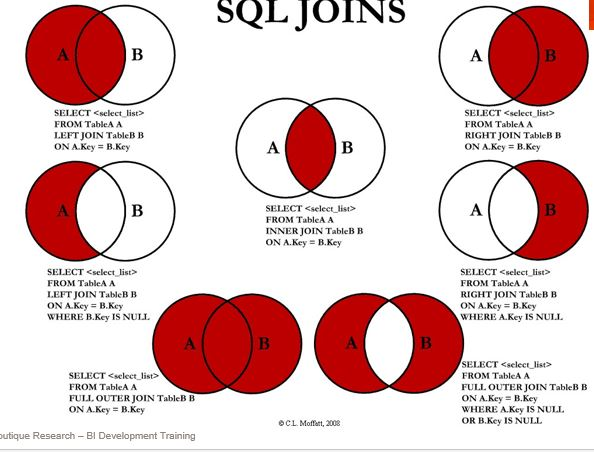
\includegraphics[width=0.6\textwidth]{week3_1}

\caption{joint table }
\end{figure}

\pagebreak
\noindent \textbf{Exercises description week 3}

\begin{itemize}
\item MySQL Exercise 4: This exercise involves summarising your data using the most common aggregate functions such as AVG,MAX,COUNT,MIN and SUM.

\item  MySQL Exercise 5: This exercise sheet focuses on grouping the data. The commands explored are GROUP BY and HAVING.
\item MySQL Exercise 6: looks at common mistakes of group by usually found in MYSQL and how to avoid them.

\item MySQL Exercise 7: This exercise involves selecting data by using inner joint with simple use of AND operators. 

\item MySQL Exercise 8: This exercise involves selecting data by using MYSQL LEFT and RIGHT joint operator. Also it shows how to achieve outer joint on MYSQL.

\item Viewpoint Interface for Teradata Queries: A series of teradata exercises where conducted. A comparison between terdata and MYSQL was shown. 
\end{itemize}

\section*{Week4}

This week you will practice integrating the SQL syntax you’ve learn so far into queries that address analysis questions typical of those you will complete as a business data analyst.\\

\textbf{Tasks learnt this week}:
\begin{itemize}
\item Design and execute subqueries.
\item Introduce logical conditions into your queries using IF and CASE statements.
\item Implement analyses that accommodate missing data or data mistakes.
\item Write complex queries that incorporate many tables and clauses.
\end{itemize}

\subsection*{Starting through your analysis plan}

Defining that a business analyst job is to do something that will clarify exactly what a business should do to solve a problem.\\

\noindent If you wish to look at start an analysis project. The first thing you do is to start an structured analysis plan. Data analysis project needs to provide insight into business processes that a business has the ability and willingness to improve in order to create new value. \\

In order for a data analyst to tackle this problem, Some questions should be considered as :
\begin{itemize}
\item What questions will provide actionable insight?
\item Will the answers to my questions matter? 
\item Are the answers to my questions correct?
\end{itemize}

The main focus will be on the last to questions that the the planning will have a big affect on the project. You may have heard the term analysis paralysis before. It's a real thing. It's what happens when you are so overwhelmed by all the ways you can analyse a data-set that you end up doing nothing at all. Even more dangerous, though, is what I call analysis free-for-all The dangers of analysis paralysis and analysis free-for-all start at the very beginning, when you want to begin playing around with the data so that you can get a feel for what they tell you.

\noindent \textbf{Exercises description week 4}

\begin{itemize}
\item MySQL Exercise 9: This exercise involves to learn how to incorporate subqueries and derived tables into our queries. Subqueries, which are also sometimes called inner queries or nested queries, are queries that are embedded within the context of another query. 

\item  MySQL Exercise 10: This exercise sheet focuses on Useful Logical Operators such as true and false and others. 


\end{itemize}


\end{document}
